\chapter{Results and Discussion \label{sec:results}}

\section{Testbed Verification \label{sec:testbedResults}}
Before the testbed was used to facilitate comparison between different SDR modules detection performance, its design and components were tested according to the steps in the methodology section. Whilst this was relatively straightforward, it was necessary to ensure the project could meet its aims of a simple, user friendly, potentially scaleable design. 

\subsection{SDR Module Verification \label{sec:sdrVerification}}
The RTL-SDR and LimeSDR Mini were tested to ensure they could be used in the testbed. This comprised of testing both the software driver functionality as mentioned in Section \ref{sec:SDRcomparison} and the hardware / communication functionality. 
% RTL SDR TESTING
\par \vspace{0.5cm}
\noindent
\textbf{RTL-SDR}
The RTL-SDR was tested using a combination of librtlsdr command line tools and GQRX, both on the mac and the Rpi5. Starting with the below command to ensure the hardware was detectable:

\begin{verbatim}
    rtl_test -t
\end{verbatim}

\noindent 
In conjunction with the antenna testing below \ref{sec:antennaVerification}, the RTL-SDR waterfall plot was obtained via GQRX, as seen in Figure \ref{fig:rtlSDRwaterfall}.

\begin{figure}[h!]
    \centering
    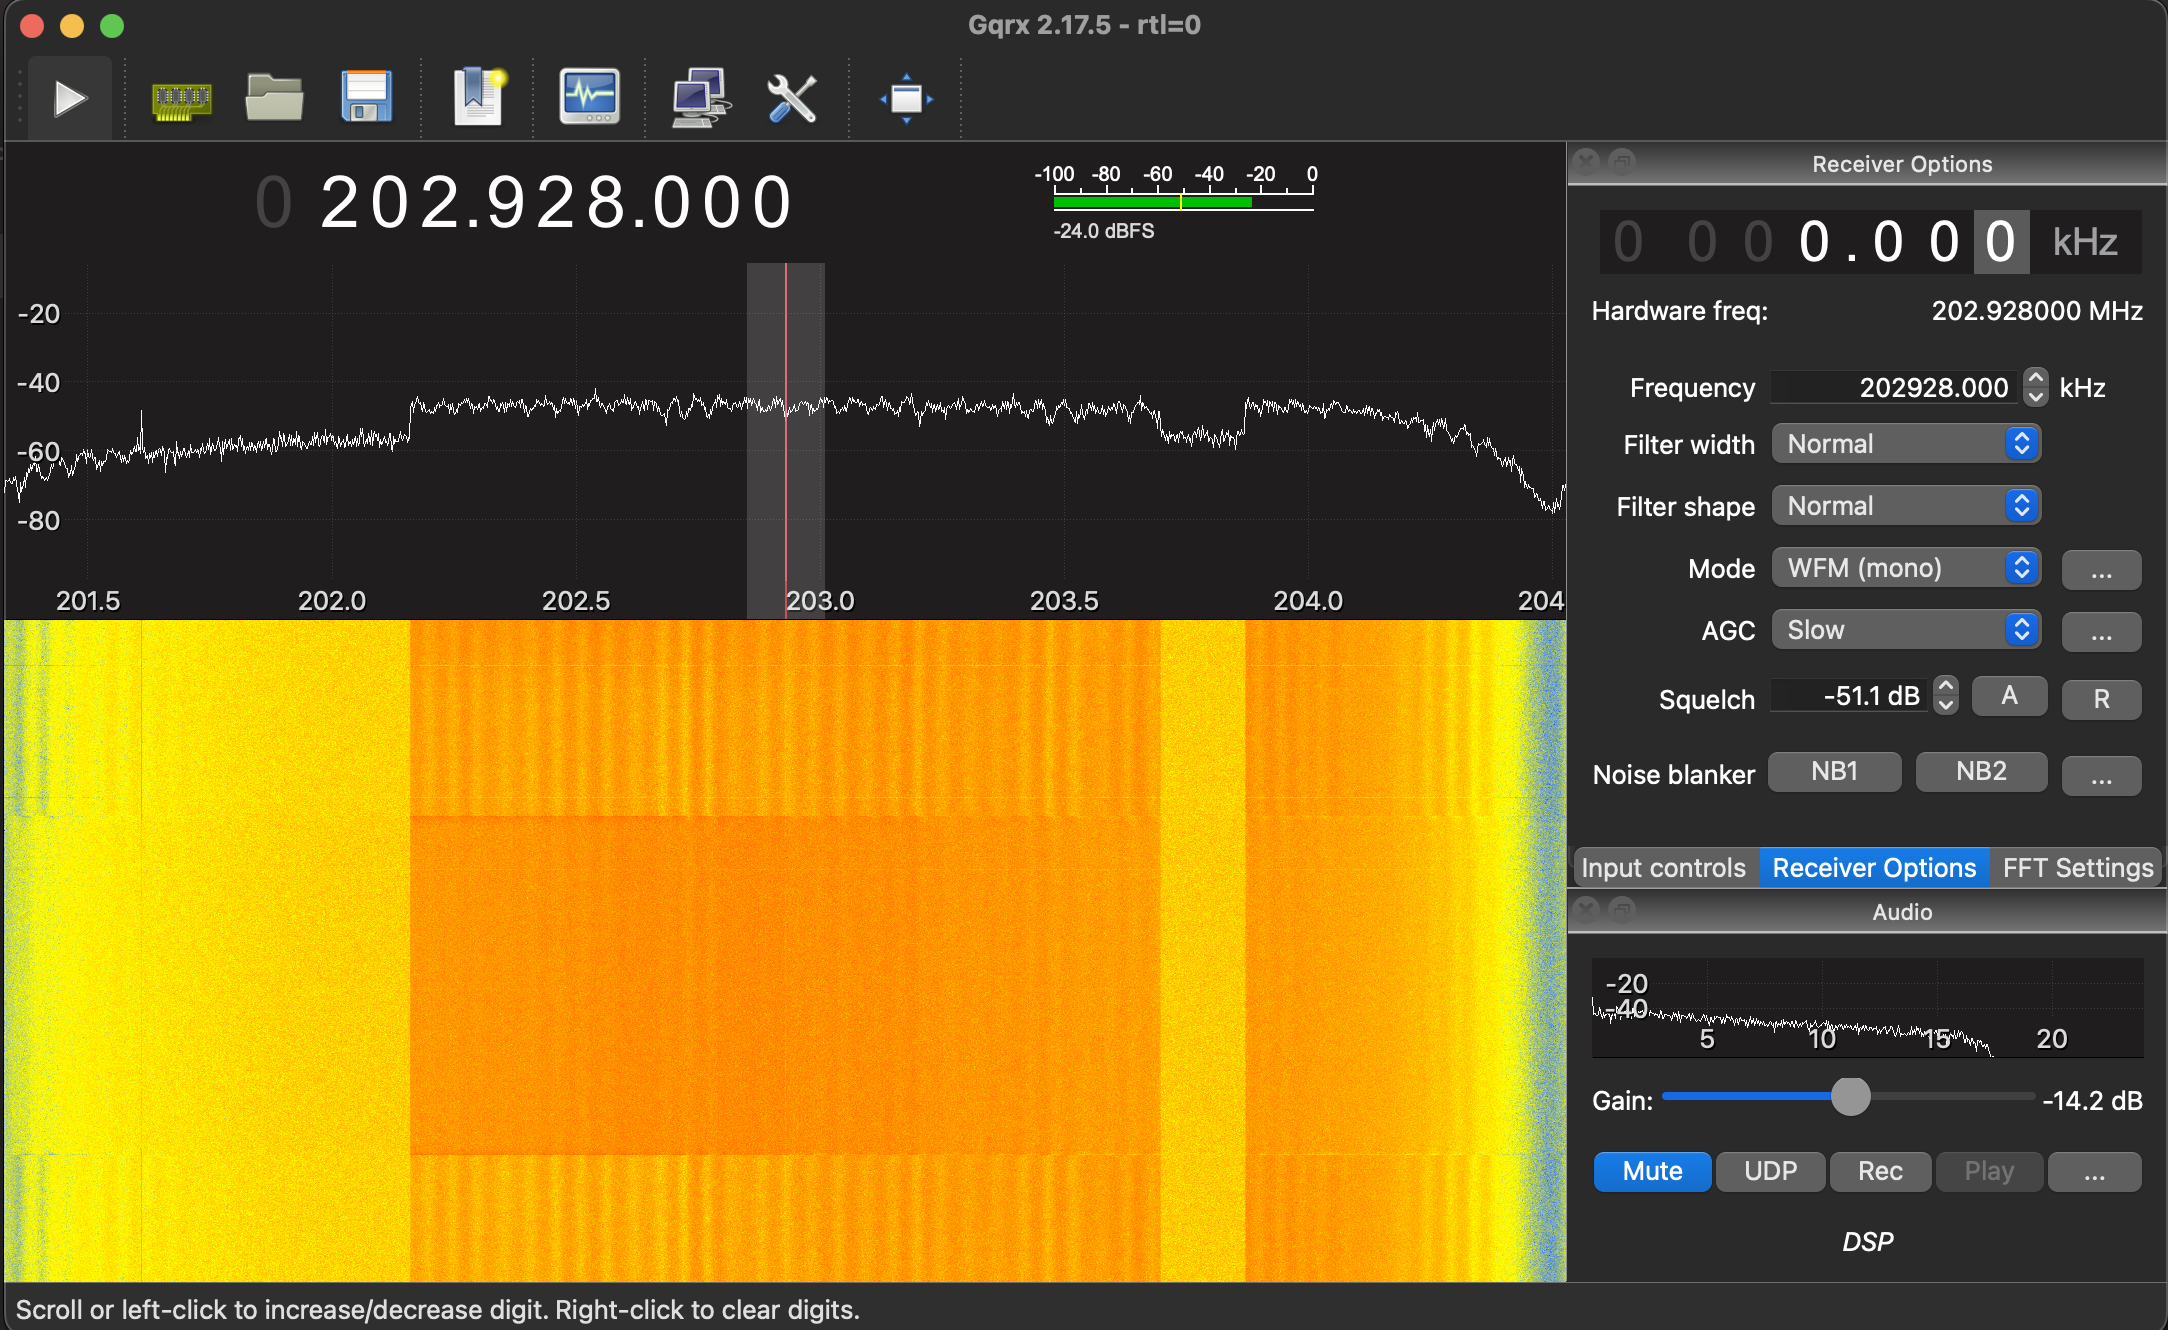
\includegraphics[width=0.6\textwidth]{smaAntennaNF.png}
    \caption{RTL-SDR Waterfall Plot (DAB Multiplex 9A)}
    \label{fig:rtlSDRwaterfall}
\end{figure}

Given that the relevant data processing was to be conducted with a python script, it was also neccessary to test the ability of the RTL-SDR to sample and output data to a .bin file. This was done using the following command:
\begin{verbatim}
    rtl_sdr -s 2048000 -f 202.928e6 -n 2048000 testData.bin 
\end{verbatim}

\noindent
The above test was successful in saving raw IQ data to a .bin file, in the executed directory. Where the saple rate was 2.048 MS/s, the centre frequency was 202.928 MHz (DAB Multiplex 9A) and the number of samples was 2048000 (1 second of data). The \textit{testData.bin} file size for the above example was 4.1MB, highlighting the importance of the storage medium as the sample time is scaled up, as discussed in Section \ref{sec:sbcVerification}.   

\par \vspace{0.5cm}
\noindent
\textbf{LimeSDR}
As with the RTL-SDR, the LimeSDR hardware and software was verified, however it required more effort to test given the relative lack of driver API's. Firstly, the hardware was tested using the Limesuite Hardware API:
\begin{verbatim}
    LimeUtil --find
    LimeQuickTest
\end{verbatim}

\noindent
Which worked to first detect the LimeSDR and then run a series of tests to ensure the hardware was functioning correctly. Specifically the quick test verfied functionality of the clock network, FPGA EEPROM, LMS7002M tuner chip, and the RF loopback. Once the physical hardware was verified it was necessary to ensure that the SoapySDR unifying API was working correctly and could detect the LimeSDR. This was done using the SoapySDRUtil command line tool and output:

\begin{verbatim}
    SoapySDRUtil --find
    ######################################################
    ##     Soapy SDR -- the SDR abstraction library     ##
    ######################################################
    Found device 0
    addr = 1d50:6108
    driver = lime
    label = LimeSDR-USB [USB 3.0] 90706024F3821
    media = USB 3.0
    module = FX3
    name = LimeSDR-USB
    serial = 00090706024F3821
\end{verbatim}

Further information about the LimeSDR and its channels was obtained using the following command:
\begin{verbatim}
    SoapySDRUtil --probe="driver=lime"
\end{verbatim}

\noindent The output of the above command can be viewed in the appendix \ref{lst: soapyProbe} and its information was used to configure the LimeSDR for sampling in the python script.

\noindent A python script was then created which utilised the SoapySDR API to sample and save data to a .bin file. The script is viewable in the Appendix \ref{app:limeSDRscript}, this was based on similar code sourced from DeepWave Digital for an Air-T SDR \cite{complexSamplingPython}. Noteably, as seen in the SoapySDR probe information \ref{lst:soapyProbe}, there was no automatic gain control for the LimeSDR RX1, therefore the low noise amplifier (LNA) gain was set to 30dB. The script was verified by saving a .bin file and then plotting the PSD of the sample, showing the DAB multiplex centered around 202.928 MHz, as seen below. 

% Image of the PSD of the LimeSDR
\begin{figure}[h!]
    \centering
    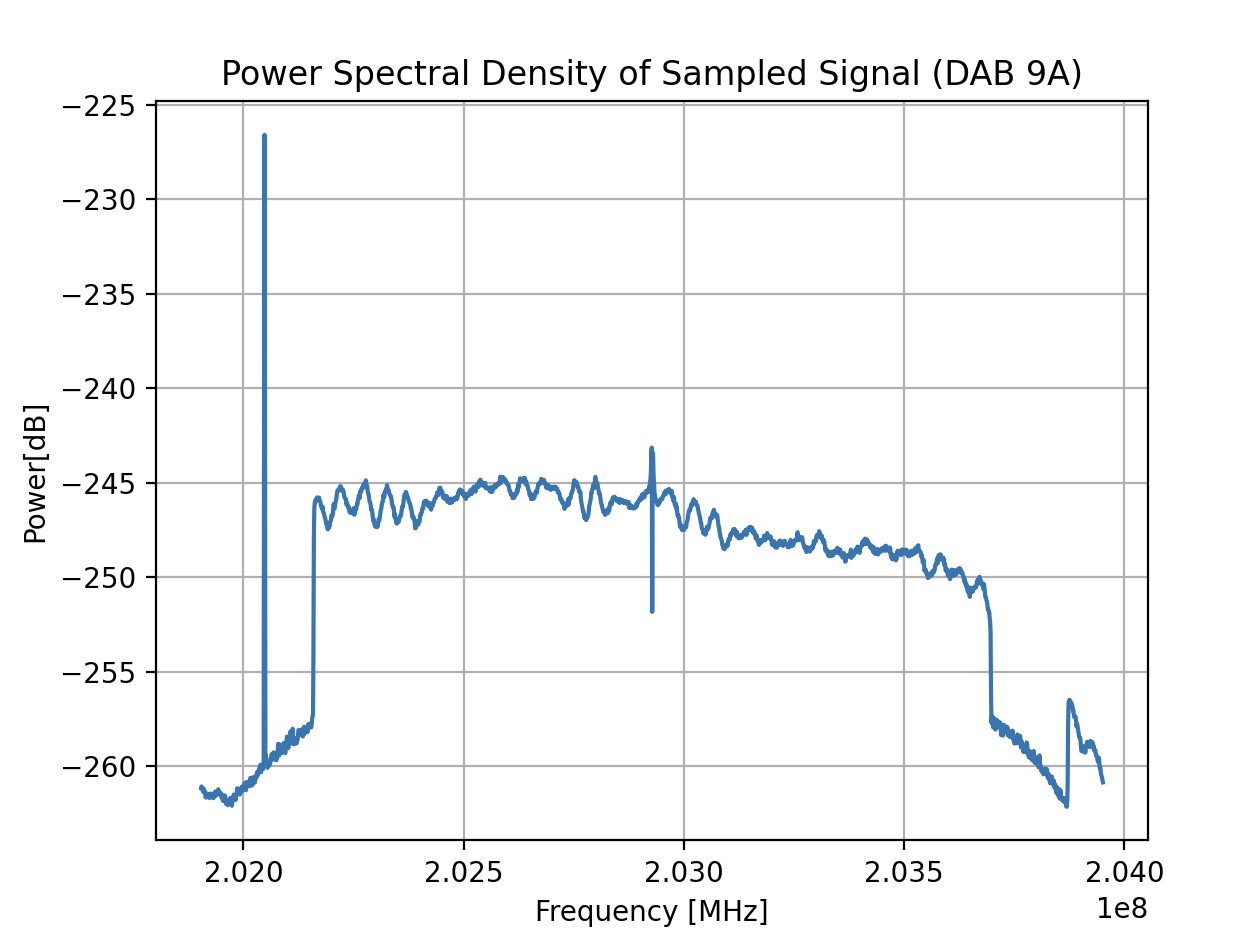
\includegraphics[width=0.6\textwidth]{LimeSDRpsd.png}
    \caption{LimeSDR PSD Plot (DAB Multiplex 9A)}
    \label{fig:limeSDRpsd}
\end{figure}

Notably, given the LimeSDR has a 12 bit ADC, the output complex IQ data is 32 bits total, with a 16 bit real and 16 bit imaginary component (12 bits zero padded at LSB). The output settings of the LimeSDR are configured via the \textit{SOAPYSDRCS16} format. This resulted in the saved .bin file being 8.2MB for 1 second of data, again showing the high storage requirements for the testbed. On the RPi5, GQRX was also able to be utilised to view the waterfall plot of the LimeSDR, as seen in Figure \ref{fig:limeSDRwaterfall}, adding an additional layer of verification, other than the python script and source libraries. 

\begin{figure}[h!]
    \centering
    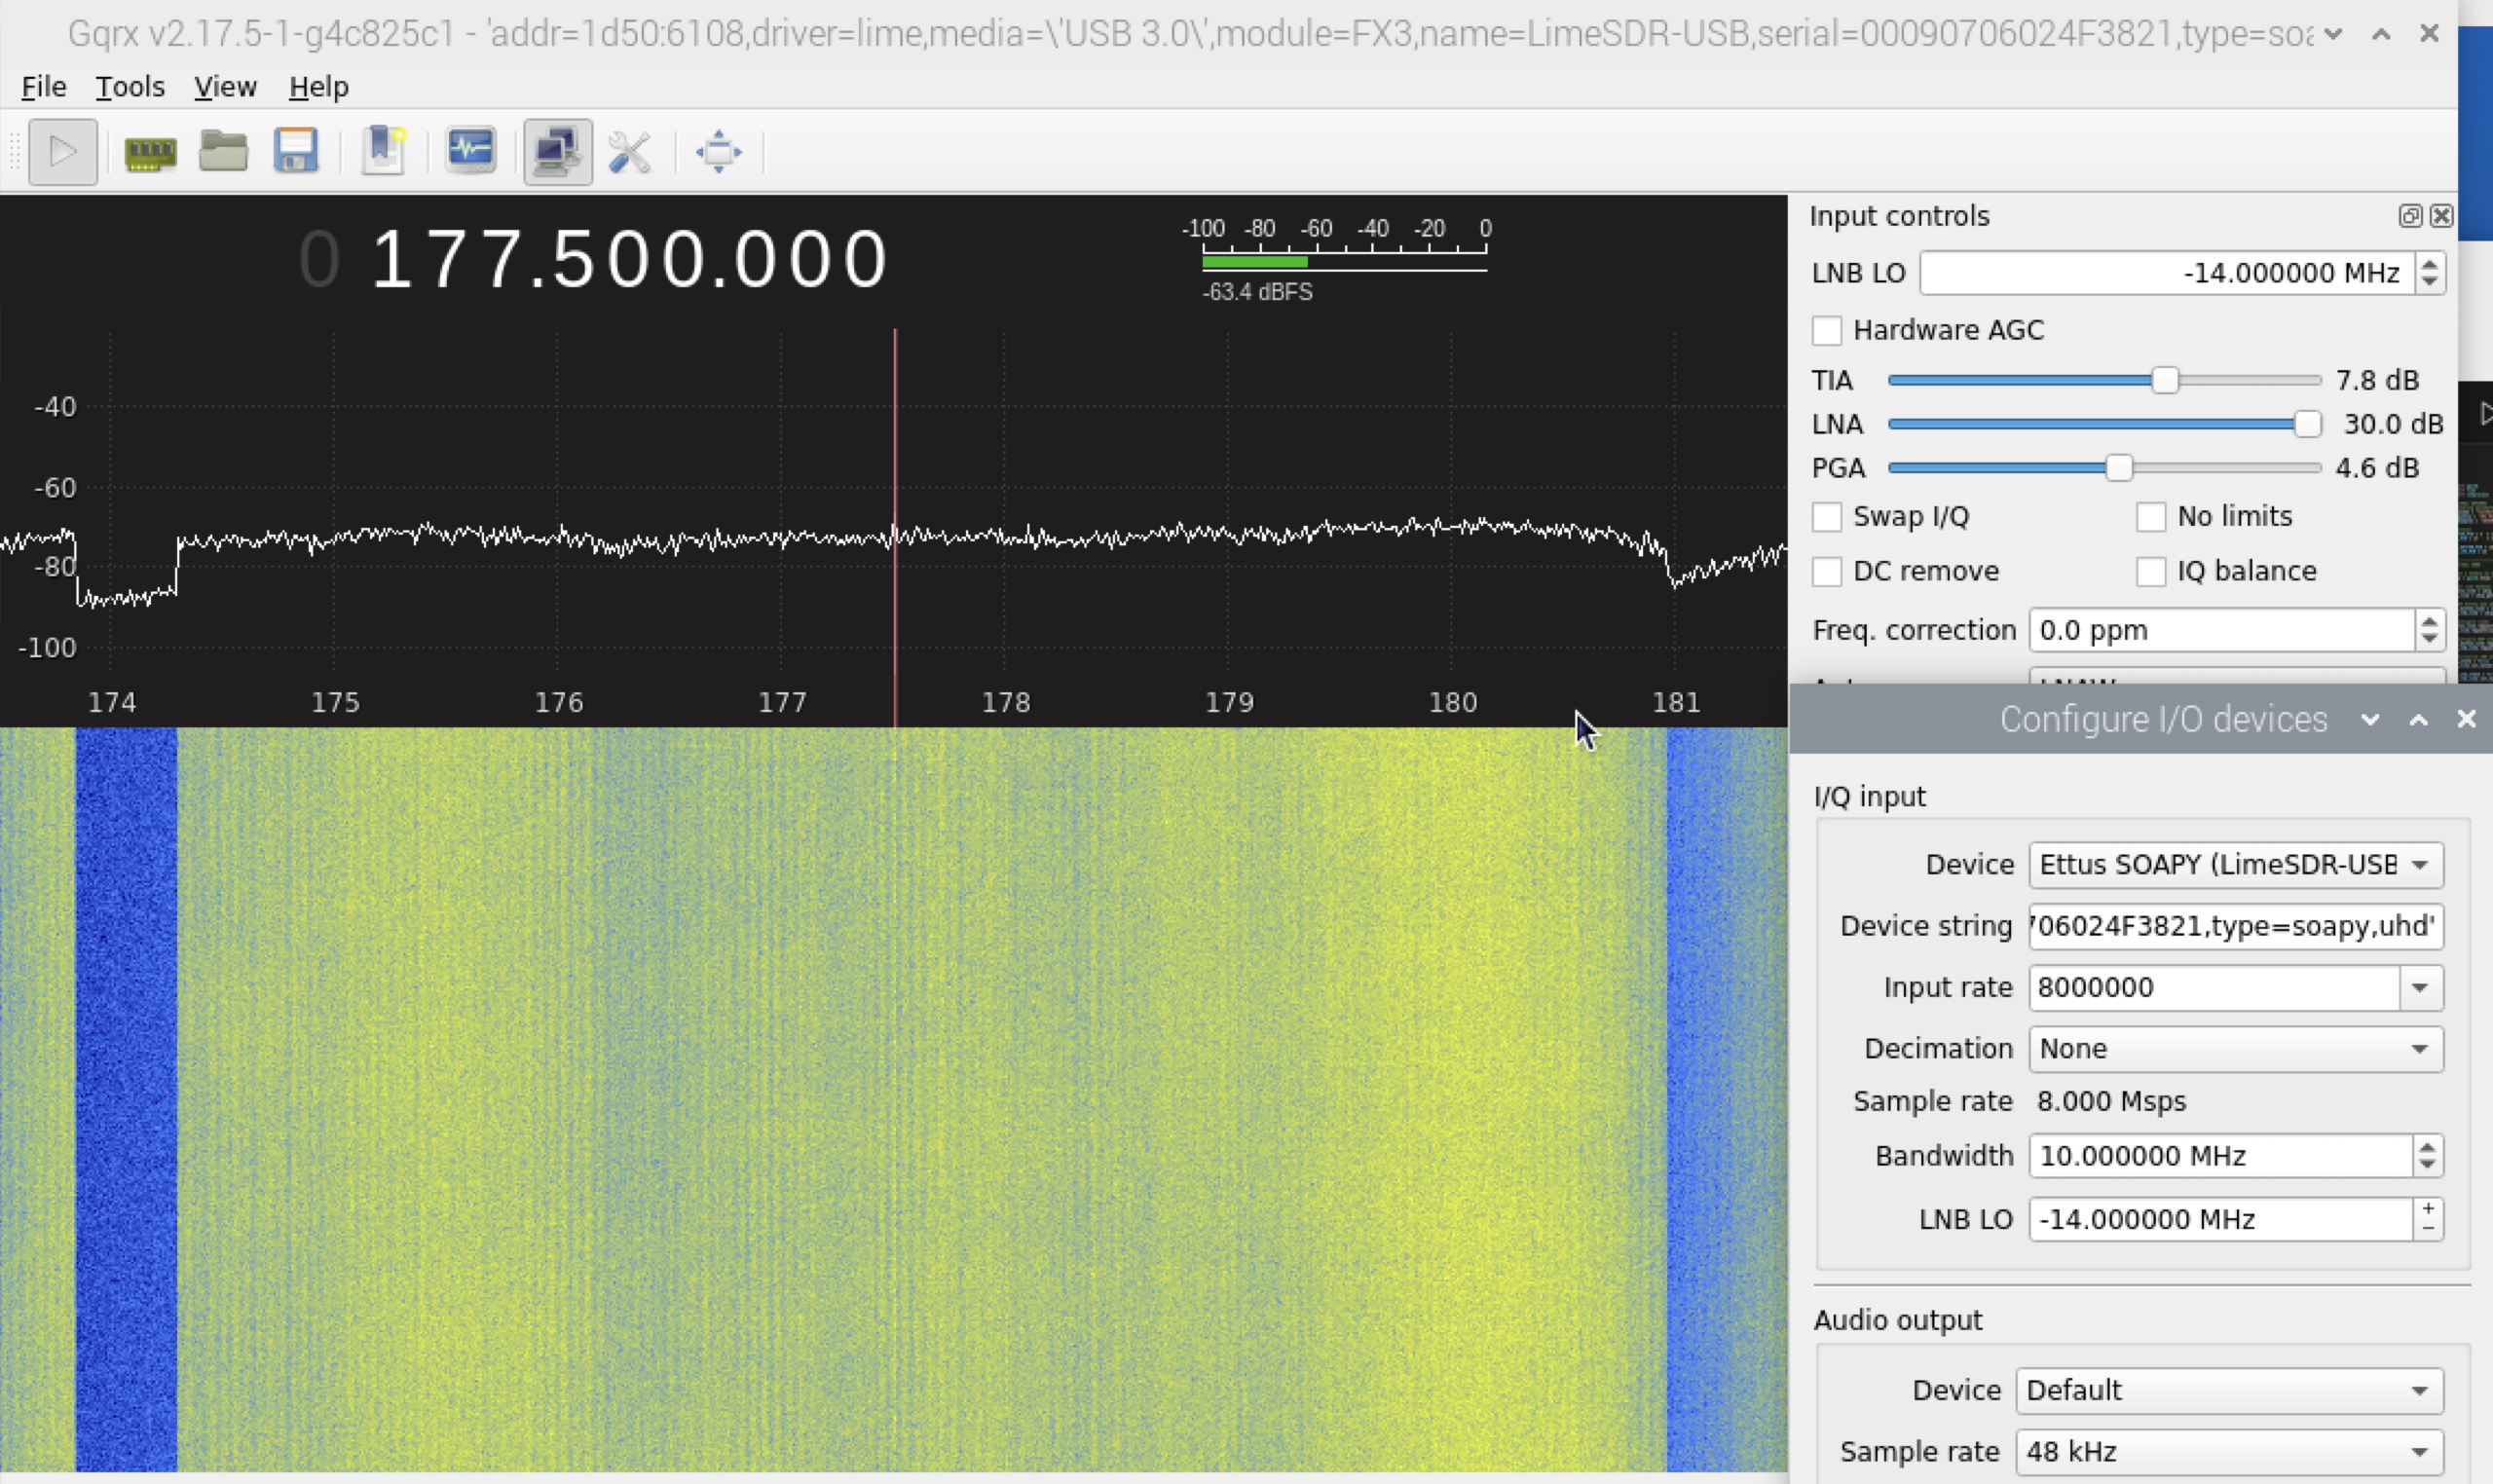
\includegraphics[width=0.8\textwidth]{DVBtLime.png}
    \caption{LimeSDR Waterfall Plot (Channel 7 DVB-T Multiplex 177.5MHz)} 
    \label{fig:limeSDRwaterfall}
\end{figure}

In figure \ref{fig:limeSDRwaterfall}, the waterfall plot shows almost 10Mhz width of spectrum bandwidth, highlighting the capability of the LimeSDR to sample a wide bandwidth of spectrum. This is in contrast to the RTL-SDR which has a maximum sample rate of 3.2MS/s, and a bandwidth of 2.4MHz. Importantly, this bandwidth and sampling rate is also variable (via source scripting or API's), and multipel different sampling rates were experimented with during testing.

\subsection{RPi5 and NVME Testing \label{sec:sbcVerification}}
In order to compare and quantify the differences in the storage performance between the microSD card and the NVME SSD, a series of tests were conducted, utilising the following linux commands via the terminal of the RPi5.

\begin{verbatim}
    lsblk
    sudo hdparm -t --direct /dev/nvme0n1 
    sudo hdparm -t --direct /dev/mmcblk0
\end{verbatim}

\noindent Resulting in the following output seen below in Table \ref{tab:diskperf}.

\begin{table}[h!]
    \centering
    \caption{Disk Read Performance: NVMe vs MicroSD Card \label{tab:diskperf}}
    \begin{tabular}{|l|l|}
    \hline
    \textbf{Device} & \textbf{Read Performance} \\ \hline
    \texttt{NVMe SSD (\texttt{/dev/nvme0n1})} & \texttt{751.22 MB/sec} \\ \hline
    \texttt{MicroSD Card (\texttt{/dev/mmcblk0})} & \texttt{84.83 MB/sec} \\ \hline
    \end{tabular}
\end{table}

The results in Table \ref{tab:diskperf} clearly show the obtained significant performance increase when using the NVME SSD compared to the microSD card. Given the large amount of data that generated and processed during the SDR sampling. 

\subsection{Antenna Testing \label{sec:antennaVerification}}

Before calculations or detection was performed, the signal strength of the received signal was measured. This was done by first using the RTL-SDR and the monopole SMA antenna and compared to the Yagi-Uda antenna. The received signal strength, representing the illuminator DAB signal, was measured approximately 6km away from the transmitter tower. The results of the signal strength measurements are shown in Table \ref{tab:signalstrength}.

\begin{table}[h!]
    \centering
    \caption{Noise Floor and SNR Comparison with -14.2 dB Gain (RTL-SDR)}
    \label{tab:signalstrength}
    \begin{tabular}{|c|c|c|c|}
        \hline
        \textbf{Antenna Type} & \textbf{Noise Floor (dB)} & \textbf{Signal Strength (dB)} & \textbf{SNR (dB)} \\ \hline
        SMA Monopole & -60 & -40.9 & 19.1 \\ \hline
        Yagi-Uda     & -60 & -17   & 43   \\ \hline
    \end{tabular}
    \vspace{0.5cm}
\end{table}

The above table reflects the high gain of the Yagi-Uda antenna, which is a directional antenna, compared to the monopole SMA antenna. Overall, this testing was valuable to benchmark a noise floor and appreciate the neccessity for a high gain antenna, especially in the context of the low power target signal.

% GEOMETRY OF TESTING - image of geometry
\begin{figure}[h!]
    \centering
    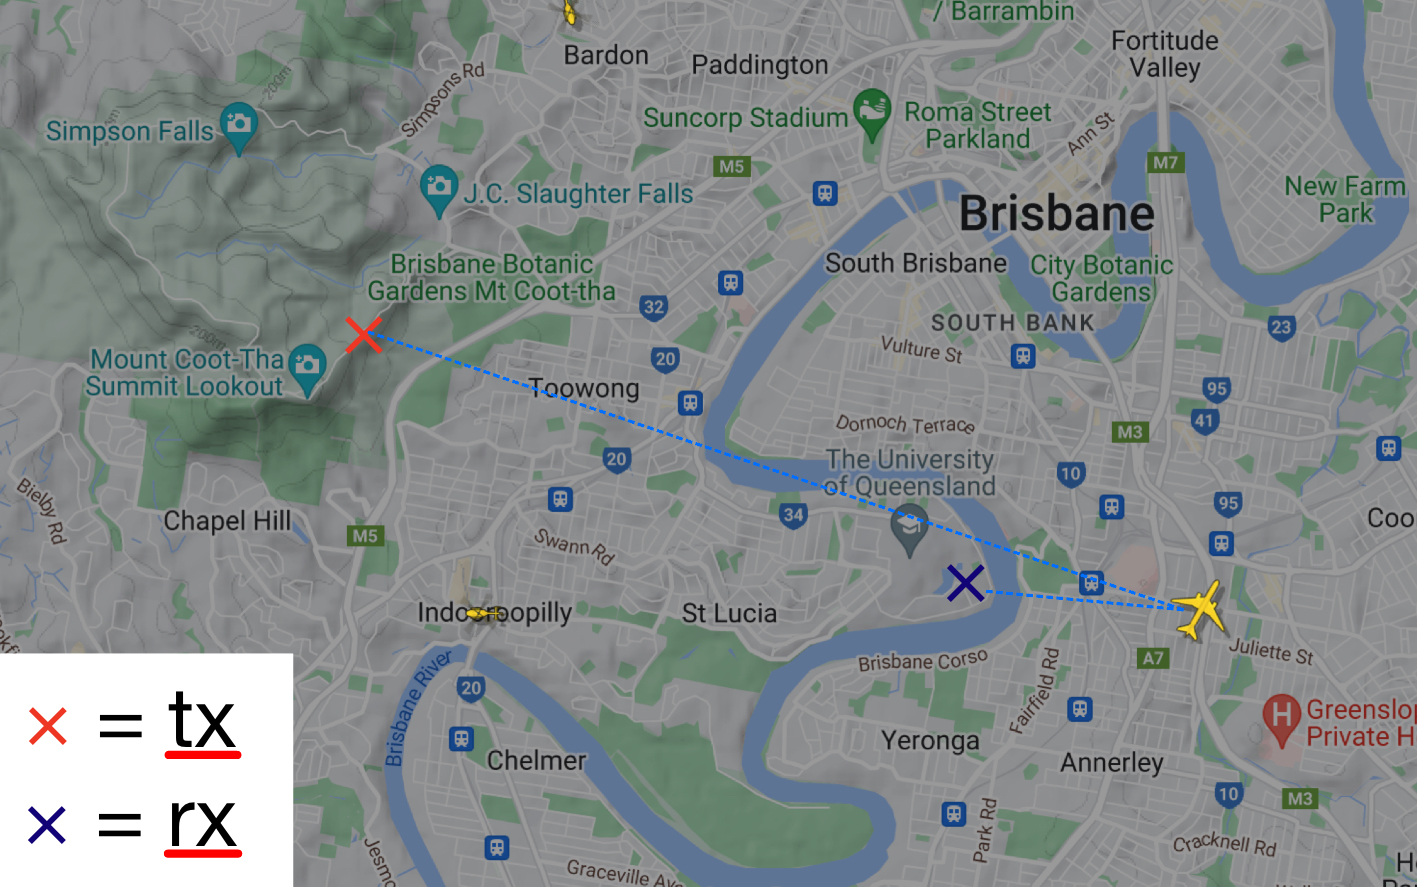
\includegraphics[width=0.9\textwidth]{testingGeometry.png}
    \caption{Antenna and Testbed Testing Geometry}
    \label{fig:antennaGeometry}
\end{figure}


\subsection{GPIO and Software Excecutable Testing \label{sec:gpioTesting}}

The GPIO buttons and LED's were tested using a simple python script, which was executed on the RPi5. The script was able to detect the button press and light the LED, as expected. This was a simple test, but was important to ensure the user interface was functioning correctly.   This was implemented via the gpiod library, which was installed on the RPi5. Specifically, the script utilised the gpiochip4 which is the GPIO chip on the RPi5. 

\par \vspace{0.5cm}
\noindent
Once basic arcade button functionality had been established, using the \textit{subprocess} library, the python script was tested executing the RTL-SDR sampling script as below:

\begin{verbatim}
    rtl_sdr_process = subprocess.Popen(['rtl_sdr', '-s', '2048000', '-f', 
    '202.928e6', '-n', '2048000', 'testData.bin'])
\end{verbatim}

\noindent This was tested with the lime SDR on the Debian baed Rpi5, and worked well. On both the Rpi5, the config/sampling and processing functionality was implemented through seperate Jupiter notebooks, for ease of use and debugging purposes along with timing and performance testing. These notebooks were migrated across to scripts for the final testbed implementation. The scripts were tested and integrated with the GPIO buttons and LED's, and the user interface was tested to ensure the user could start and stop the data collection and processing. In order to ensure execution at boot/run time on the Rpi5, the main testbed python script was configured via a \textbf{crontab} entry, which was tested and verified, and is viewable in the appendix. The efficacy of tis was tested via running the below command after boot:
% ADd code of crontab entry
\begin{verbatim}
    ps -ef | grep python
\end{verbatim}

The python script that is run by the crontab essentially polls the latch user buttons, and then sample and compute the data appropriately. The code for the python script and the crontab entry can be viewed in the appendix \ref{lst:crontab}.

\subsection{Detection Edge Processing Comparison} \label{sec:edgeProcessing}
Other than some configuration changes, the processing scripts for M1 Mac and the Rpi5 were essentially the same, revolving around range doppler processing windows of 500K samples. The figure below shows the processing time for the M1 Mac and the Rpi5, with the Rpi5 taking approximately 6 times longer to process the same amount of data.

\begin{figure}[h!]
    \centering
    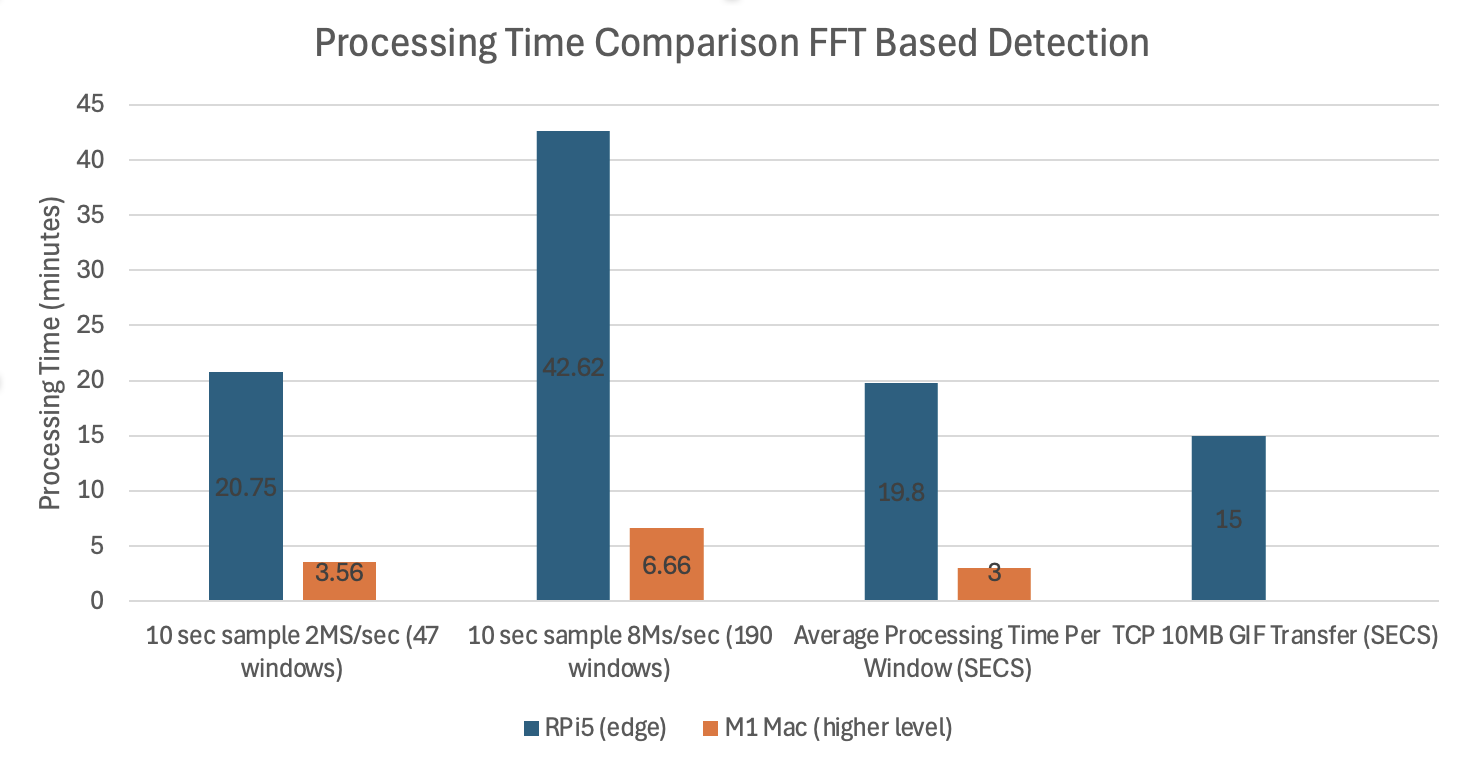
\includegraphics[width=0.75\textwidth]{timeComparison.png}
    \caption{Processing Time Comparison}
    \label{fig:processingTime}
\end{figure}

The difference above is as expected, given the M1 Mac has a 8 core CPU and 16GB of RAM, compared to the Rpi5 which has a 4 core CPU and 8GB of RAM. The results highlight how networking the .bin files to a more powerful computer for processing could be a potential solution to the Rpi5's processing limitations.

\subsection{Enclosure Creation} \label{sec:enclosureResults}
Once the functionality of the testbed was verified, the enclosure was designed and 3D printed. The case design was modelled off source code from \cite{RPiCase}, however it was necessary to enhance the original design with cutouts for the user buttons and also stretch the top of the case to accomodate the SMA connectors and buttons. 

% Image of the enclosure design
\begin{figure}[h!]
    \centering
    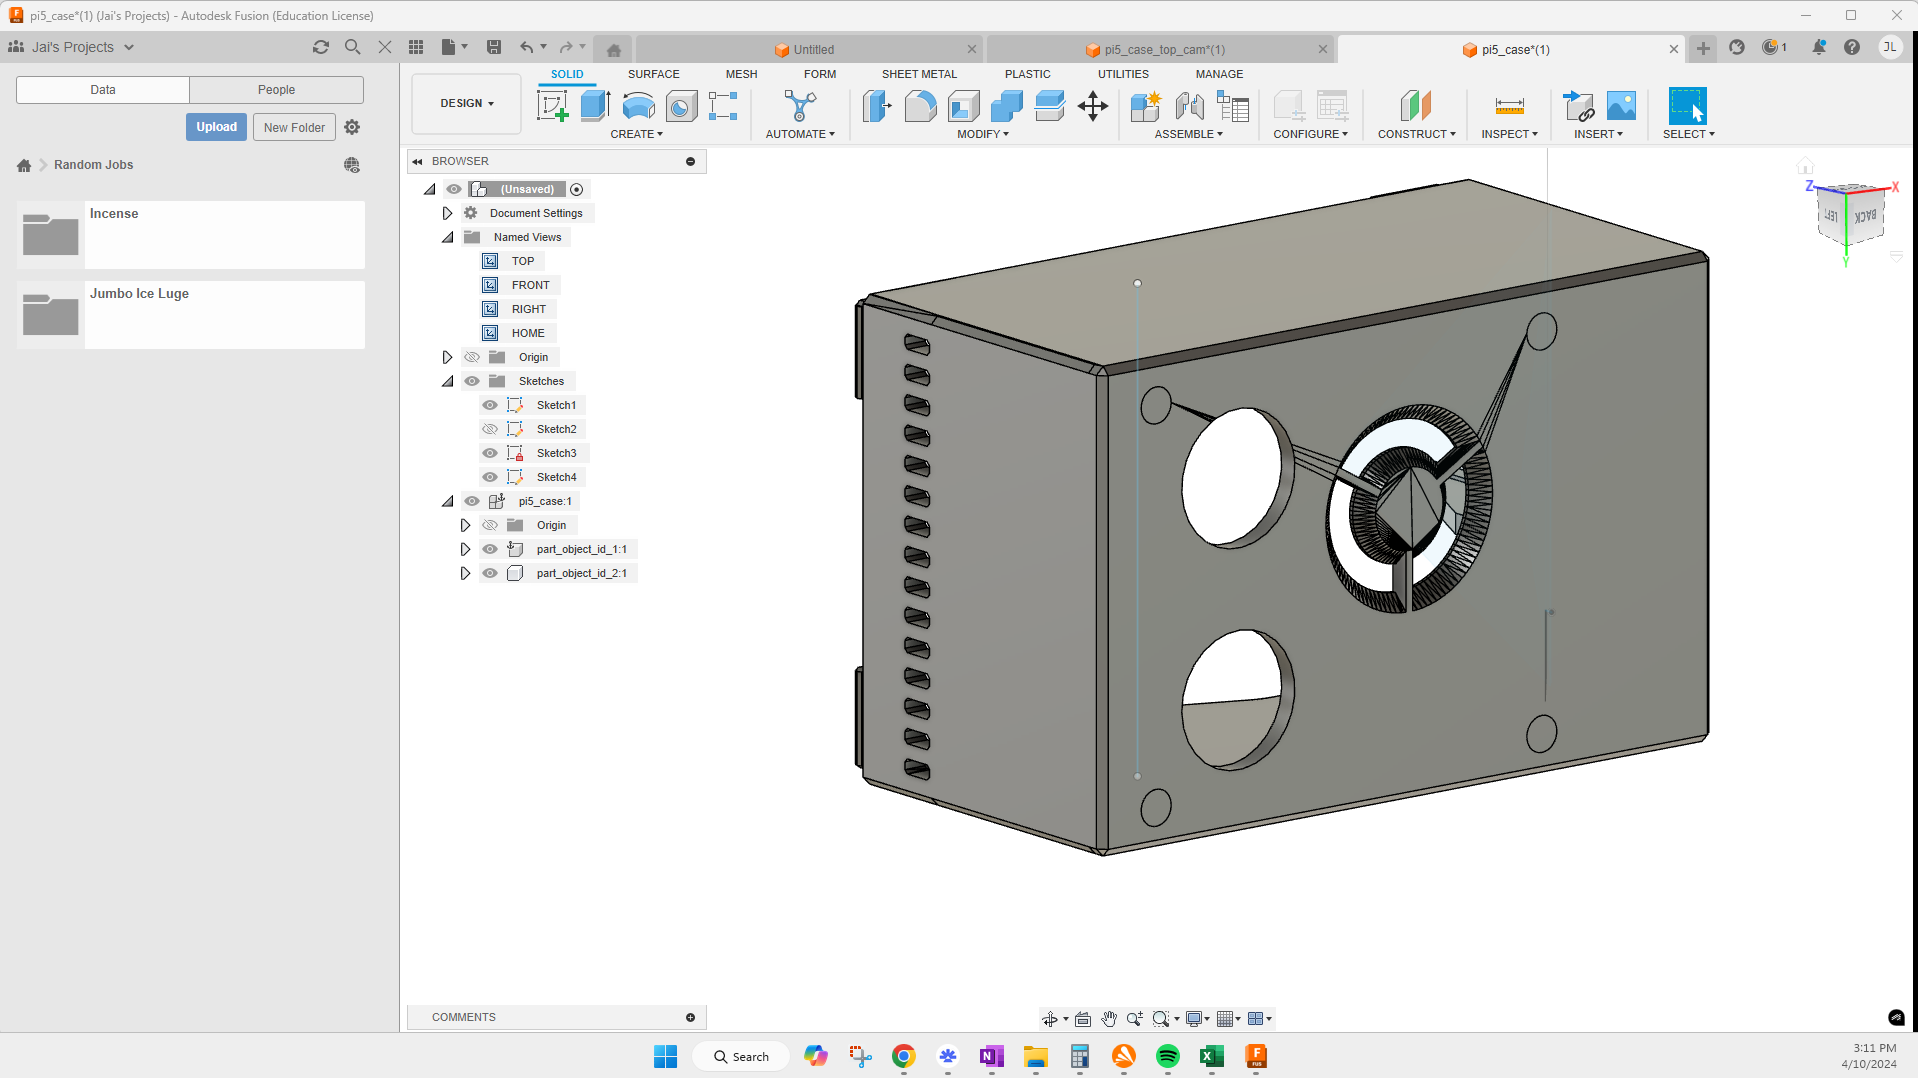
\includegraphics[width=0.8\textwidth]{RPiCase.png}
    \caption{Enclosure Design}
    \label{fig:enclosureDesign}
\end{figure}

Fusion 360 was used to design the case, and the STL files were then 3D printed. The design of the final case design can be seen in Figure \ref{fig:enclosureDesign}. The case was printed using a Bambu Lab P1S 3D printer, utilising the default PLA filament, which is not ideal given the potential heat generated by the RPi5 and the LimeSDR. The case was printed in two parts, the top and the bottom, and then assembled. However, given the active and passive cooling requirements of the RPi5 and the LimeSDR, it was deemed fit for purpose.


\section{RTL-SDR vs LimeSDR Detection Comparison \label{sec:SDRcomparison}}
RTL-SDR detection was performed via the testbed first and yielded successful detection results despite lack of clutter suppression and zero doppler cancellation. LimeSDR range doppler mapping was attempted unsuccessfully due to presence of overwhelming zero doppler clutter. 

\subsection*{RTL-SDR Detection}
Firstly, the FFT algorithm was conducted on 15 seconds of RTL-SDR data, with the DAB signal at 202.928 MHz. The first specific flight was QF936, a Boeing737 on 7 October 2024. The flight path and range doppler maps are shown in Figure \ref{fig:QF936}.

\begin{figure}[h!]
    \centering
    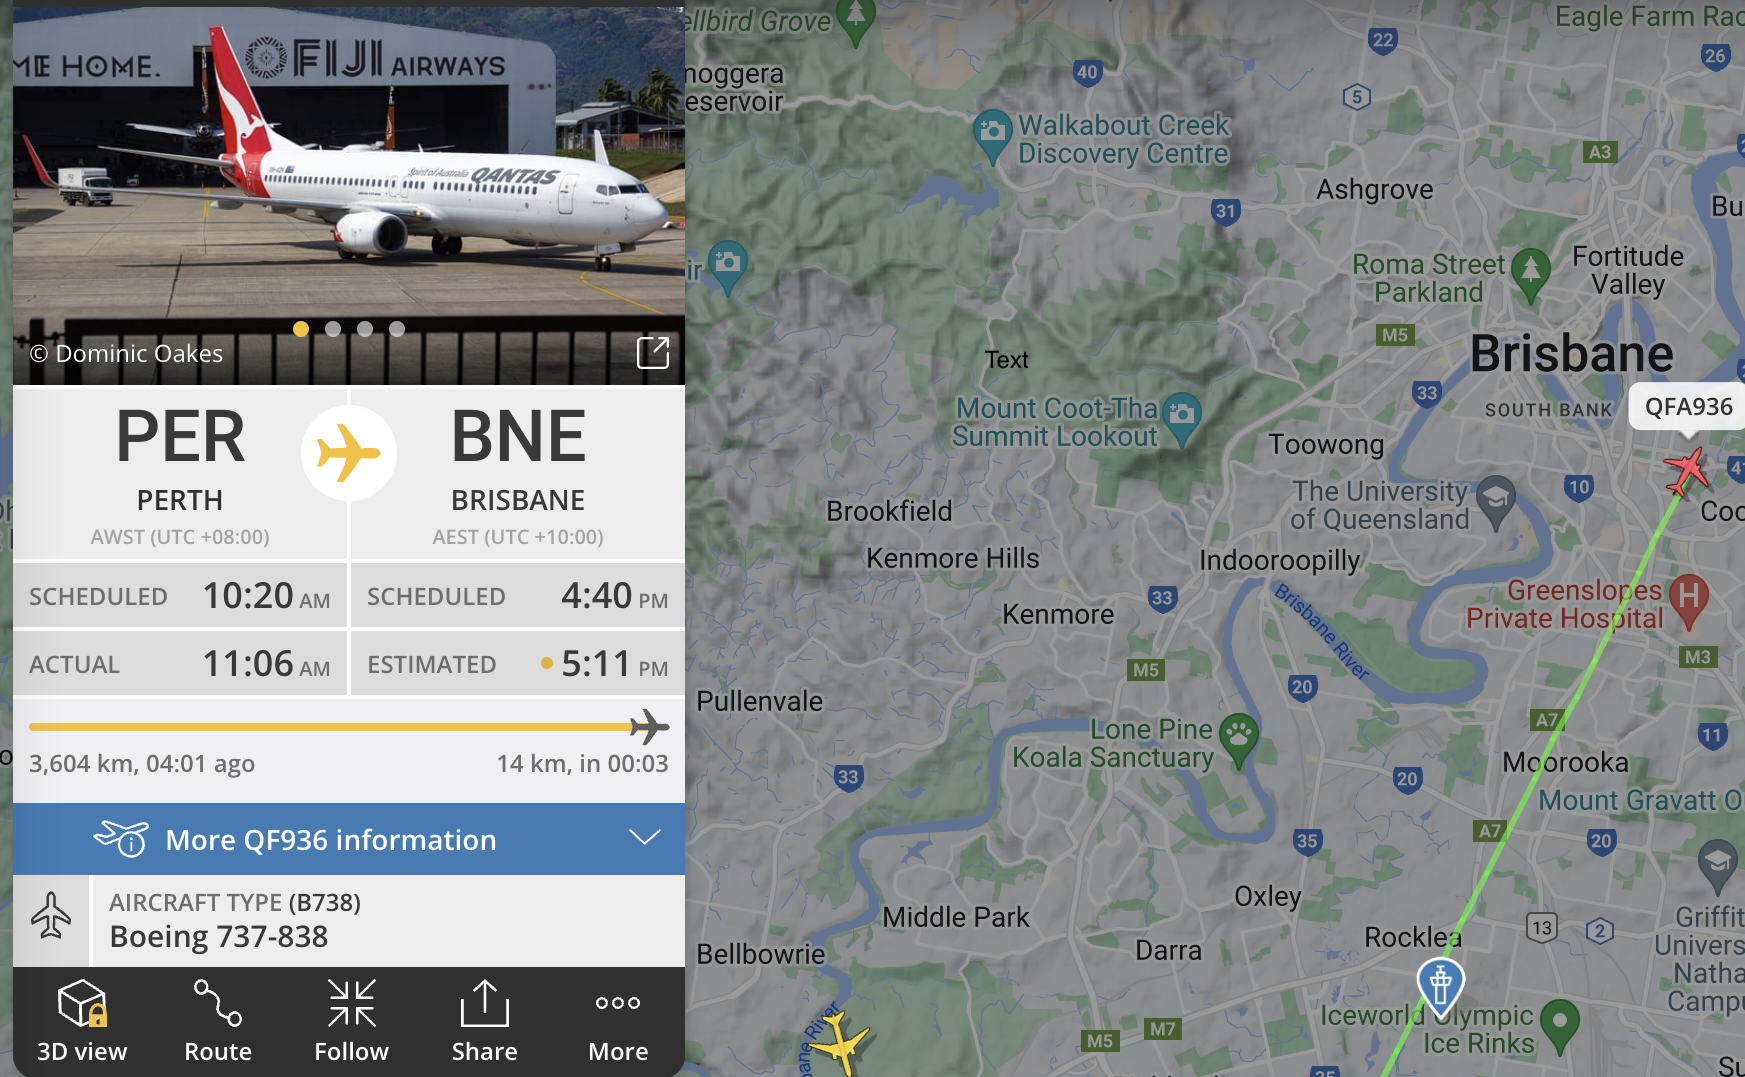
\includegraphics[width=0.6\textwidth]{firstGoodFlight.png}
    \caption{QF936 Flight Path \cite{flightradar24}}
    \label{fig:QF936}
\end{figure}

\begin{figure}[h!]
    \centering
    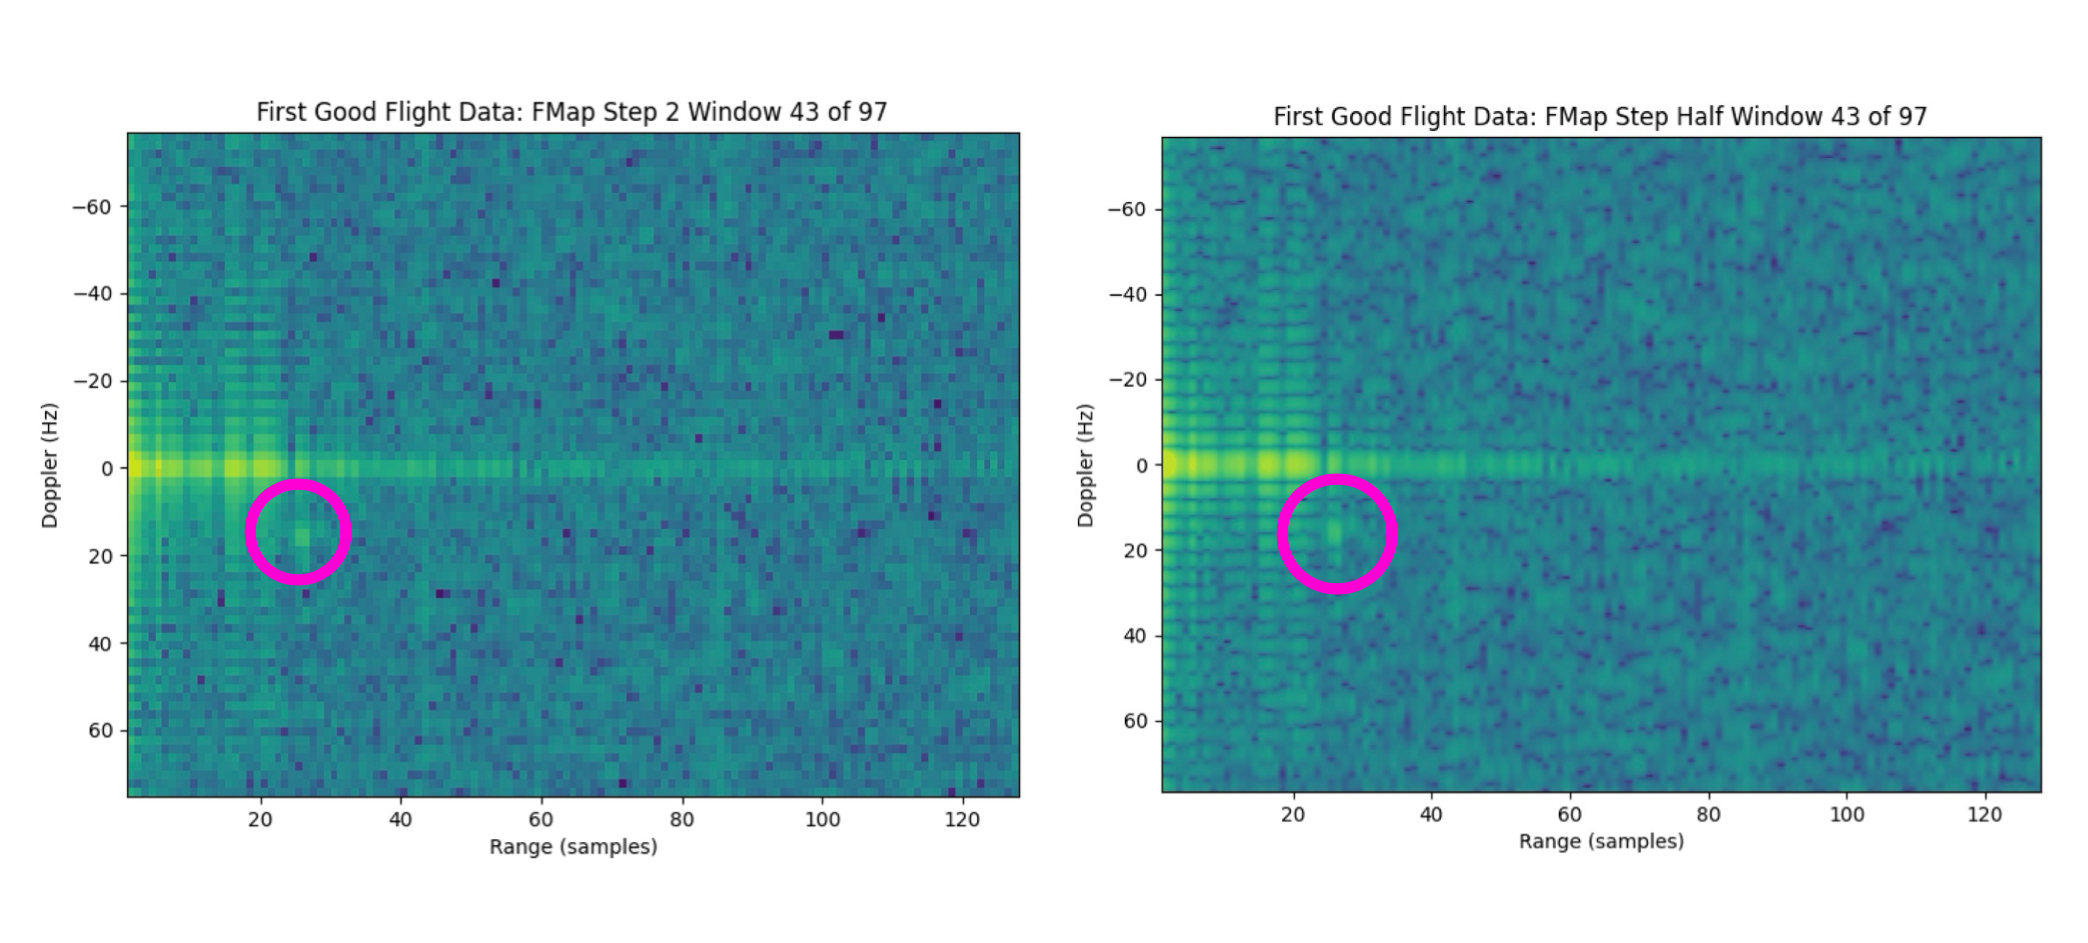
\includegraphics[width=0.99\textwidth]{RangeDopplerGoodFlight1.jpeg}
    \caption{FFT Method Range Doppler Output: Frequency Bin Step Size Comparison}
    \label{fig:RDM1}
\end{figure}

The GIFs of the detection over the space of 97 windows, and can be viewed in further detail in the appendix \ref{sec:codeResults}. In terms of understanding the range doppler map, detection at around the 25th sample bin refects a detection range of approximately 1.8km, which is consistent with the flight path of QF936. Furthemore, the doppler shifts from postive (moving towards the receiver) to negative (moving away from the receiver) at around the 50th sample bin, which is consistent with the flight path of QF936. The signal was sampled as tested in Section \ref{sec:sdrVerification}, with a sample rate of 2.048 MS/s, and a centre frequency of 202.928 MHz, using the automated gain control (AGC) of the RTL-SDR.

\subsection*{LimeSDR Detection}
In the same test location, a range of samples were taken of passing targets on the LimeSDR, starting with a sample rate of 2000Mhz, the below range doppler map was generated in Figure \ref{fig:RDM2}. 

\begin{figure}[h!]
    \centering
    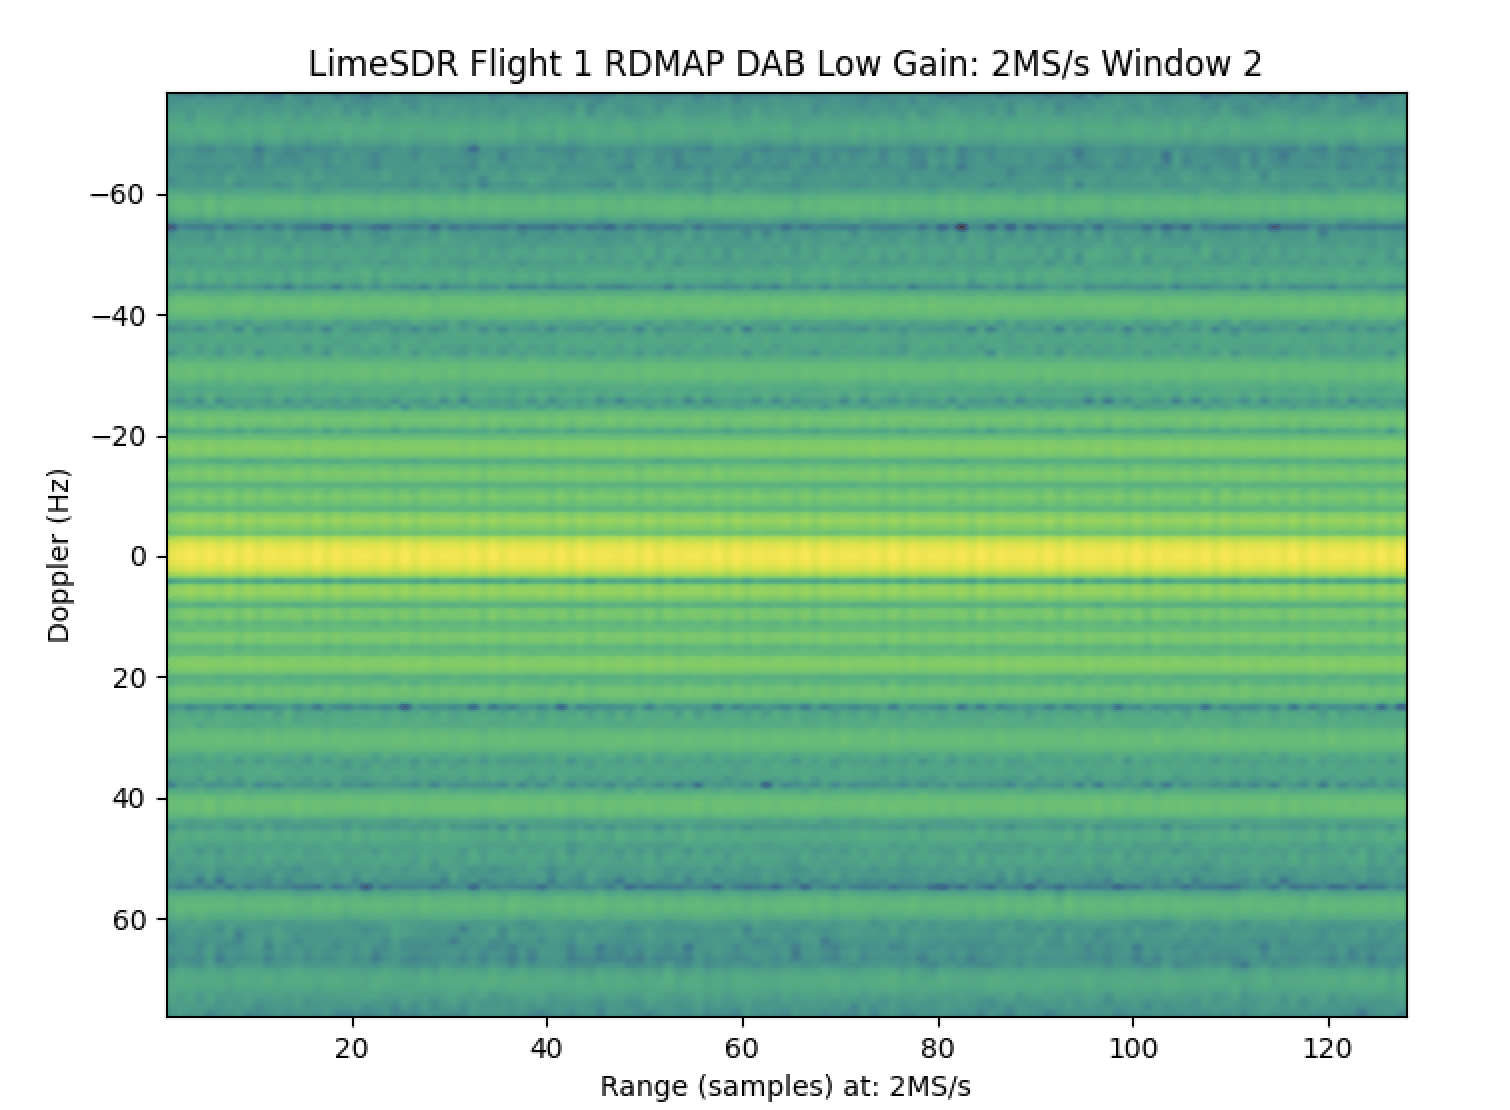
\includegraphics[width=0.89\textwidth]{LimeSDRdabLow.png}
    \caption{LimeSDR Medium Gain Range Doppler Output: Noisy Clutter}
    \label{fig:RDM2}
\end{figure}

The horizontal noise bands indicate a significant amount of zero doppler clutter, which is interesitng given the RTL-SDR did not have this issue. The LimeSDR was configured using an LNA gain of 20dB, and a PGA gain of 5dB. The gain was increased when attempting to detect a target to no avail, with the range doppler map in Figure \ref{fig:RDMLimeHighGain}. 

\begin{figure}[h!]
    \centering
    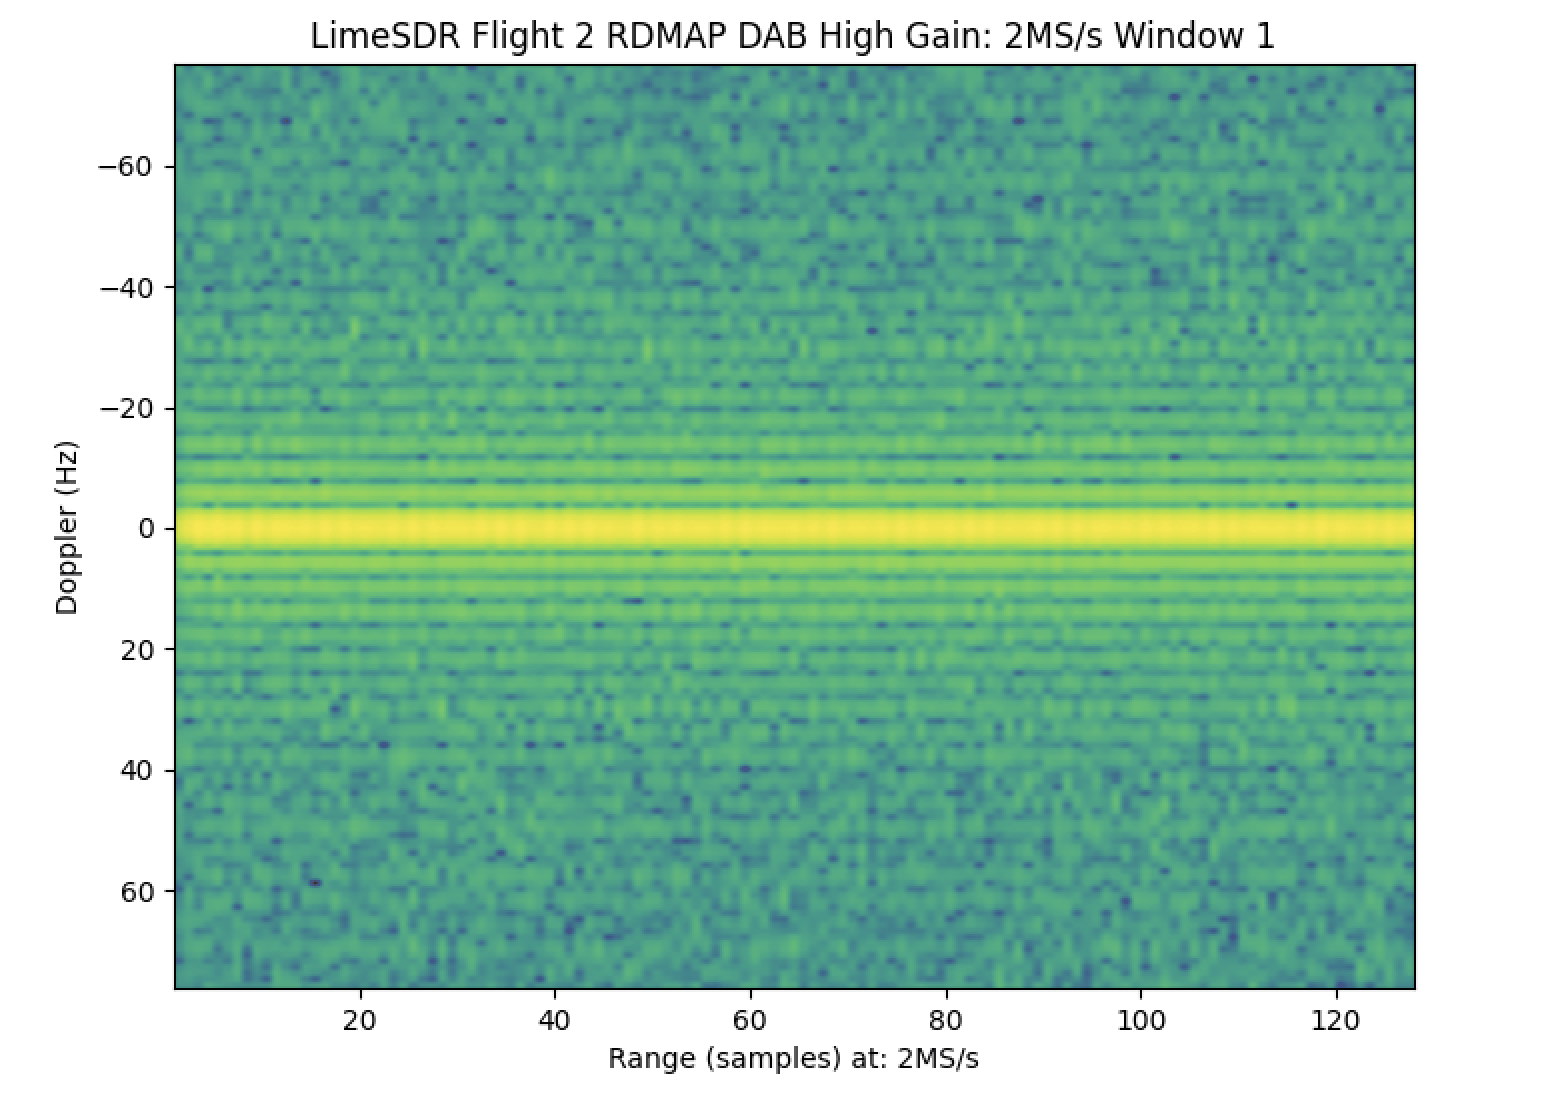
\includegraphics[width=0.69\textwidth]{LimeSDRdabHigh.png}
    \caption{LimeSDR DAB High Gain Range Doppler Output: Noisy Clutter}
    \label{fig:RDMLimeHighGain}
\end{figure}

Despite being in the same location, the SNR of the LimeSDR was significantly lower than the RTL-SDR, which can potentially be attributed to the lack of AGC. A different illuminator signal was then utilised (DVB-T 177.5MHz), along with a higher sampling rate (bandwidth) of 8000Mhz, and the range doppler map in Figure \ref{fig:RDMLimeDVB} was generated.

\begin{figure}[h!]
    \centering
    \includegraphics[width=0.69\textwidth]{DVBtLimeFlight1.png}
    \caption{LimeSDR Medium Gain Range Doppler DVB-T}
    \label{fig:RDMLimeDVB}
\end{figure}

Whilst still not being able to effectively detect passing aerial targets from the same locatiion as the RTL-SDR, the generated range doppler map in Figure \ref{fig:RDMLimeDVB} shows more expected features such as clutter around the zero range as expected with autocorellation. 


\section{Overall Design Cost}
The functioning test bed can broadly be broken down into the following components and their costs, with the only variance being the cost of the SDR module. The resulting cost: 

\begin{multicols}{2}
    \begin{itemize}
        \item Raspberry Pi5 (8GB RAM): \$135 \cite{core_electronics_rpi5}
        \item Pimoroni NVME Base: \$40 \cite{pimoroni_nvme_base}
        \item NVME Compatible SSD: \$30 
        \item RTL-SDR: \$30 \cite{RTLSDRchipSet}
        \item User Buttons: \$10
        \item Custom Case PLA: \$5 
        \item VHF / UHF Yagi Antenna: \$80 \cite{AntennaPiece}
        \item LimeSDR USB 3.0 (no longer retail): \$550 AUD \cite{limesdr_usb}
    \end{itemize}
\end{multicols}

The image below shows the final testbed, with the LimeSDR and the RTL-SDR connected to the RPi5.

\begin{figure}[h!]
    \centering
    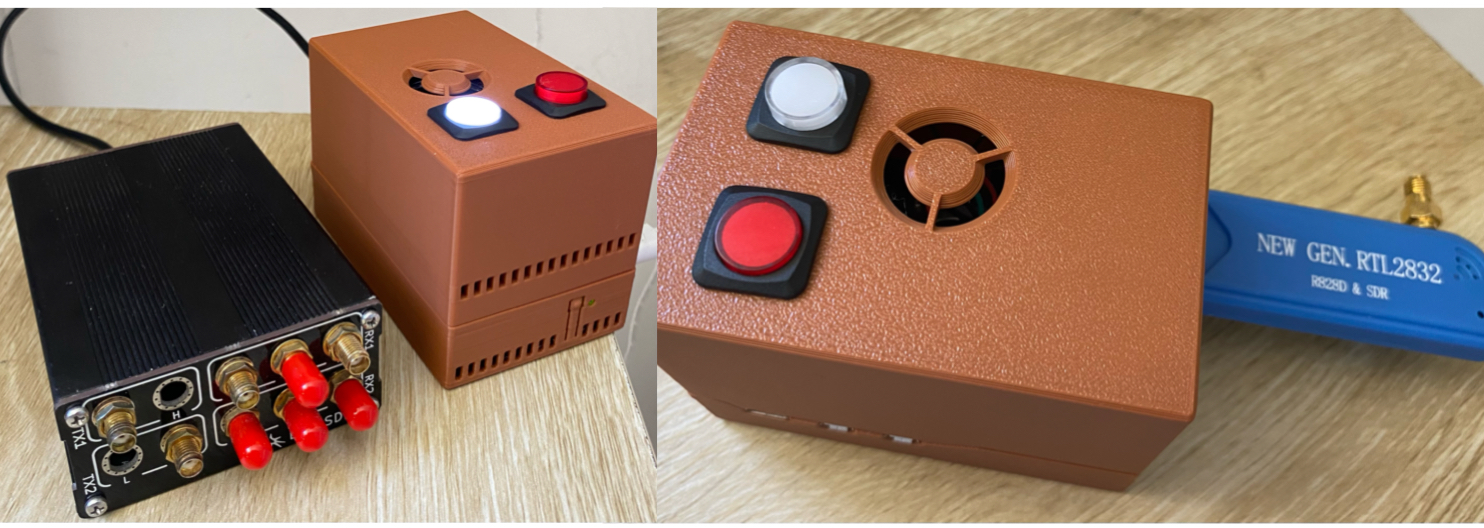
\includegraphics[width=0.8\textwidth]{testBedFinal.jpeg}
    \caption{Final Testbed}
    \label{fig:finalTestbed}
\end{figure}

This resulted in a final cost for each of the configurations:
% listed options 1 and 2
\begin{enumerate}
    \item RTL-SDR Configuration: \$330
    \item LimeSDR Configuration: \$850
\end{enumerate}


\section{Comparison to Existing Work}
To examine the implementation of the testbed along with its SDR/bandwidth comparison, it was necessary to compare it to pre-existing work. The closest work to the testbed was the work conducted by Moser et. al \cite{IOTpassiveRadar} as seen in the literature review \ref{sec:lowCostIOT}, which utilised a Raspberry Pi 3 and an RTL-SDR to detect DAB signals. The work conducted by Moser et. al was a proof of concept, and the testbed developed in this thesis was a more user friendly, scaleable version of the same concept. Analsyis and comparison of these results and that of Moser et al. (the Moser study) inclue:

% List of comparisons
\begin{itemize}
    \item \textbf{Hardware} Both projects utilised Raspberry Pi, with this project using the latest and updated Model. This project extended the Moser study via the addition of a higher level and cost LimeSDR. Overall, this study slightly higher in cost due to updated Pi and testbed additions such as higher speed NVME base. 
    \item \textbf{Illuminator Signal} The Moser study explored both anlaogue FM along with DAB, this study focused on digital signals only, similarly with a single channel setup. 
    \item \textbf{Signal Processing} This study did not focus on optimising already existing autocorrelation algorithms, rather demonstrating the ability to detect the signal with the RTL-SDR and LimeSDR. Moser was able to show real time detection on the Rpi3 via the batch algorithm, which based on extrapolation would be possible on the Rpi5. The utilisation of a single channel configuration saved a lot of the synchronisation and matched filtering required for the FM multichannel configuration. The compute of the fourier transform correlation method was actually larger than that of Moser, wiht the Batch implementation. Interestingly, Moser provided a real time threshold value for computations, demonstrating the ability to exceed this with the Rpi3 and batch algorithm, even demonstrating potential for additional CFAR processing.
    \item \textbf{Detection} Both studies demonstrate successful detection, however the Moser study provides a third axis on the colourless range doppler map, highlighting the signal dBFS (relative to full scale). The Moser study applied some filtering which slightly reduced noise, probably comparible to the zero range bin removal of this study. 
\end{itemize}

Overall, despite differences in result comparison, noticeably the Moser study emphasing hardware compute modules, and this study looking at different SDR modules. The Moser study provided a good benchmark for the capabilities of low cost IoT hardware in PBR applications, allowing this study to further the proof of concept with modernised hardware around a similar price tag. Both show that for sub \$300 USD, a passive radar detection system can be implemented, a range of signals can be utilised, and aerial targets can quite easily be detected with minimal additional processing.

% KRAKEN SDR COMPARISON
The next logical comparison is with both clutter suppression implementations and angle of arrival detection implementations. The KrakenSDR ecosystem is an example of full suite (close to) passive radar utilising five RTL-SDR tuners, with built in synchronisation. This off the shelf product (essentially a setup) comes with the preloaded open source API's preconfigured, and retails for approximately \$500usd \cite{KrakenSDR}.
\par With clutter evidently present in \ref{fig:RDM1}, another comparison can be made with the work of Zhang et. al \cite{ZhangClutter}, who implemented a range of clutter suppression algorithms such as BMS, GMS and CFAR. The work of Zhang et. al was able to detect smaller, further away targets, along with multiple targets in the space of one sample window.